
%========================================================================================
% Lecture 3: Aggregate Demand and Aggregate Supply (AD–AS)
% Uses the user's SimpleDarkBlue beamer template style.
% Figures are loaded from the directory: figureAD/
%========================================================================================

\documentclass[aspectratio=169,xcolor=dvipsnames]{beamer}
\usetheme{SimpleDarkBlue}

\usepackage{hyperref}
\usepackage{graphicx}

% --- Figure inclusion ---
\usepackage{booktabs}
\usepackage{appendixnumberbeamer}
\usepackage{amsmath}
\usepackage{iftex}

% --- Font handling: compile with pdfLaTeX here; switch to LuaLaTeX locally if desired ---
\ifPDFTeX
  \usepackage[T1]{fontenc}
  \usepackage{lmodern}
  \usepackage{microtype}
\else
  \usepackage{fontspec}
  \usepackage{luatexja}
  \setmainfont{Alegreya Sans Light}[
    ItalicFont={* Italic},
    BoldFont={Alegreya Sans Medium},
    BoldItalicFont={Alegreya Sans Medium Italic}]
  \setsansfont{Alegreya Sans Light}[
    ItalicFont={* Italic},
    BoldFont={Alegreya Sans Medium},
    BoldItalicFont={Alegreya Sans Medium Italic}]
\fi

% ------------ %
% beamerbutton %
% ------------ %
\newcommand{\goto}[2]{\hyperlink{#2}{\beamergotobutton{#1}}}
\newcommand{\return}[2]{\hyperlink{#2}{\beamerreturnbutton{#1}}}
\newcommand{\extgoto}[2]{\href{#2}{\beamergotobutton{#1}}}

% ------------------------------------ %
% Section title page with Huge bf text %
% ------------------------------------ %
\AtBeginSection[]{
  \begin{frame}[noframenumbering, plain]
    \Huge{\centerline{\textbf{\insertsection}}}
  \end{frame}
}

%%% automatically add spaces into enumerate and itemize environment
\let\tempone\itemize
\let\temptwo\enditemize
\renewenvironment{itemize}{\tempone\addtolength{\itemsep}{\fill}}{\temptwo}
\let\tempa\enumerate
\let\tempb\endenumerate
\renewenvironment{enumerate}{\tempa\addtolength{\itemsep}{\fill}}{\tempb}


%%=============================================================
%%  FOOTLINE TEMPLATE
%%=============================================================
\defbeamertemplate*{footline}{shadow theme}{%
    \leavevmode\hbox{%
        \hypersetup{linkcolor=white,urlcolor=white,citecolor=white}
        \begin{beamercolorbox}[wd=1.02\paperwidth, ht=2.5ex, dp=1.125ex, leftskip=.3cm plus1fil, rightskip=0.3cm]{author in head/foot}%
            \insertsectionnavigationhorizontal{.80\textwidth}{}{} \hspace{.3cm} \hfill \#\ \insertframenumber \ / \ \inserttotalframenumber%
        \end{beamercolorbox}%
    }%
}
\setbeamertemplate{footline}[shadow theme]

%----------------------------------------------------------------------------------------
%    TITLE PAGE
%----------------------------------------------------------------------------------------
\title[Lecture 3: AD--AS]{Intermediate Macroeconomics II\\\vspace{4pt}Lecture 3: Aggregate Demand and Aggregate Supply}
\author[Hui-Jun Chen]{Hui-Jun Chen}
\institute[]{National Tsing Hua University}
\date{Spring 2026}

% Figures provided by the user
\graphicspath{{figureAD/}{./}}

%----------------------------------------------------------------------------------------
%    PRESENTATION SLIDES
%----------------------------------------------------------------------------------------
\begin{document}

%------------------------------------------------
\begin{frame}[plain,noframenumbering]
    \titlepage
\end{frame}

%------------------------------------------------
\begin{frame}{Why we need AD--AS after IS--LM}
\begin{itemize}
\item \textbf{Lecture 2 result:} IS--LM determines \textbf{aggregate demand} --- a mapping from the price level (or inflation) to output.
\item But IS--LM alone cannot answer: \textbf{when does demand show up as higher $Y$ vs higher prices?}
\item \textbf{Lecture 3 goal:} add an aggregate supply block so we can talk about
\begin{itemize}
\item inflation vs output movements (demand shocks vs supply shocks),
\item short run vs medium run (adjustment back toward ``full employment'').
\end{itemize}
\end{itemize}

\vspace{0.3em}
\textbf{Big picture:}
\begin{itemize}
    \item \textbf{AD} tells us ``how much the economy wants to buy,''
    \item \textbf{AS} tells us ``how much the economy can produce.''
\end{itemize}
\end{frame}

%------------------------------------------------
\begin{frame}{Learning objectives (what you should be able to do)}
\begin{enumerate}
\item Read an AD--AS diagram and translate it into economic language.
\item Explain \textbf{what shifts AD} (fiscal policy, monetary policy, expectations).
\item Explain \textbf{what shifts AS} (productivity, labor supply, cost shocks).
\item For each shock, predict the sign of changes in $(Y,\pi)$ and the policy rate.
\item Identify the key lesson: \textbf{demand vs supply} shocks have different inflation-output comovement.
\end{enumerate}
\end{frame}

%%------------------------------------------------
%\begin{frame}{Roadmap: what each set of figures is doing}
%\begin{enumerate}
%\item \textbf{AD from IS + monetary policy:} derive the AD curve in $(\pi, Y)$ space
%\begin{itemize}
%\item Figures: \texttt{figAD0}, \texttt{figAD1}, \texttt{figAD2}
%\end{itemize}
%\item \textbf{AS from the RBC supply block:} re-plot full-employment output in $(\pi, Y)$ space
%\begin{itemize}
%\item Figures: \texttt{figAS}, \texttt{figAS1}, \texttt{figAS2}
%\end{itemize}
%\item \textbf{Put them together:} AD--AS equilibrium and comparative statics
%\begin{itemize}
%\item Figures: \texttt{figADAS}, \texttt{figADAS1--figADAS4}
%\end{itemize}
%\end{enumerate}

%\vspace{0.3em}
%\textbf{Reading rule:} every figure answers one question: \emph{which curve shifts, and what happens to $(Y,\pi)$?}
%\end{frame}

%------------------------------------------------
\section[Demand]{Demand side: IS--MP $\Rightarrow$ AD}

%------------------------------------------------
\begin{frame}{From IS--LM to IS--MP (modern central banks)}
\begin{itemize}
\item In Lecture 2 we used \textbf{LM} (money market equilibrium) to link $Y$ and the interest rate.
\item In practice, modern central banks usually implement policy by \textbf{setting an interest rate}, not by fixing money growth.
\item So we summarize monetary policy with a simple rule (an ``MP curve''):
\[
r_t = \bar r + \phi_\pi \,\pi_t \qquad (\phi_\pi>0).
\]
\item Intuition: when inflation rises, the central bank raises the real interest rate.
\end{itemize}

\vspace{0.3em}
\textbf{Why we do this:} it lets us draw aggregate demand directly in $(\pi,Y)$ space.
\end{frame}

%------------------------------------------------
\begin{frame}{Step 1: IS as a goods-demand relation}
\begin{itemize}
\item IS collects $(Y,r)$ combinations that clear the goods market.
\item In this RBC-style benchmark, higher $r$ discourages current spending, so goods demand is decreasing in $r$.
\item We will not solve IS in full detail today; we use only its direction:
\begin{itemize}
\item \textbf{Lower $r$} $\Rightarrow$ \textbf{higher goods demand} $\Rightarrow$ higher equilibrium $Y$.
\end{itemize}
\item When fiscal policy changes (e.g., $G\uparrow$), desired spending shifts and the IS relation shifts.
\end{itemize}

\vspace{0.3em}
\textbf{Key message:} IS tells you how output responds when the real interest rate moves.
\end{frame}

%------------------------------------------------
\begin{frame}{Step 2: Combine IS with MP to get AD}
\begin{itemize}
\item MP tells us how $r$ responds to inflation: $r_t=\bar r+\phi_\pi\pi_t$.
\item IS tells us how $Y$ responds to $r$.
\item Putting them together gives a relationship between inflation and output:
\[
\text{IS} + \text{MP} \quad\Rightarrow\quad \textbf{AD: } \pi \mapsto Y.
\]
\item Why AD slopes down here:
\begin{itemize}
\item higher $\pi$ $\Rightarrow$ MP raises $r$,
\item higher $r$ reduces spending $\Rightarrow$ lower $Y$.
\end{itemize}
\end{itemize}

\vspace{0.2em}
\textbf{Reading rule:}\quad along AD, \emph{inflation is higher because policy is er, so output is lower}.
\end{frame}

%------------------------------------------------
\begin{frame}{AD curve (IS--MP--AD)}
\begin{columns}[onlytextwidth,T]
\begin{column}{0.5\textwidth}
\centering
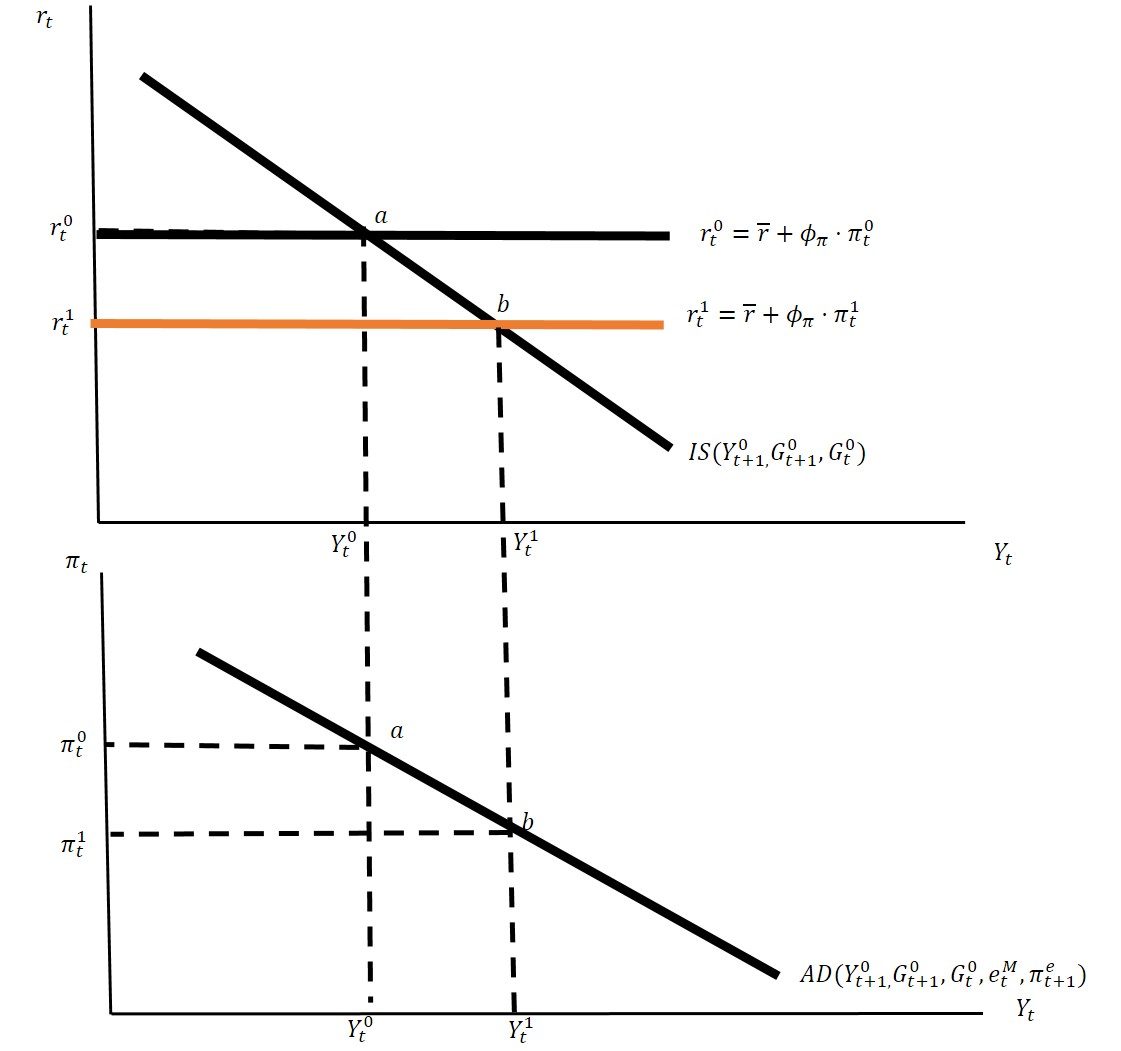
\includegraphics[width=\linewidth]{figAD0.jpg}
\end{column}
\begin{column}{0.5\textwidth}
\begin{itemize}
\item \textbf{What this figure is doing:} re-draw demand equilibrium in $(\pi,Y)$ space.
\item \textbf{Mechanism (one line):} $\pi\uparrow \Rightarrow r\uparrow$ (MP) $\Rightarrow Y\downarrow$ (IS).
\item \textbf{So AD slopes downward.}
\item \textbf{What is held fixed:} fiscal stance and the policy rule parameters $(\bar r,\phi_\pi)$.
\end{itemize}

\vspace{0.3em}
\textbf{Key message:}\quad AD is a \emph{policy-dependent} demand curve.
\end{column}
\end{columns}
\end{frame}

%------------------------------------------------
\begin{frame}{AD shifts right when government spending increases}
\begin{columns}[onlytextwidth,T]
\begin{column}{0.5\textwidth}
\centering
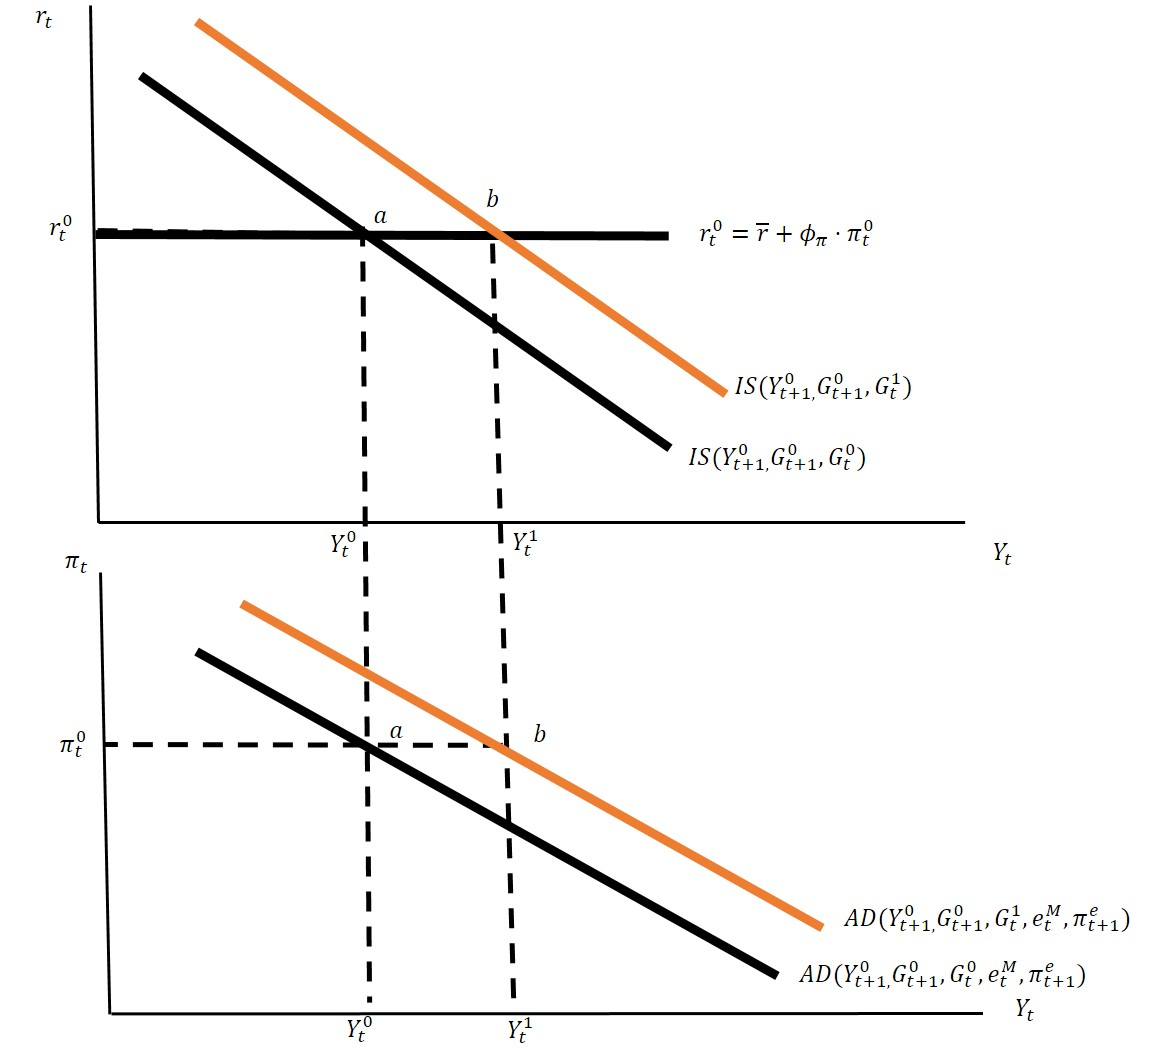
\includegraphics[width=\linewidth]{figAD1.jpg}
\end{column}
\begin{column}{0.5\textwidth}
\begin{itemize}
\item \textbf{Shock:} $G\uparrow$ increases desired spending.
\item \textbf{IS shifts:} at any given $r$, goods demand is higher.
\item \textbf{AD implication:} for a given $\pi$ (hence given $r$ from MP), equilibrium $Y$ is higher.
\end{itemize}

\vspace{0.3em}
\textbf{Key message:}\quad fiscal expansion shifts AD to the right.
\end{column}
\end{columns}
\end{frame}

%------------------------------------------------
\begin{frame}{AD shifts right when monetary policy becomes easier}
\begin{columns}[onlytextwidth,T]
\begin{column}{0.5\textwidth}
\centering
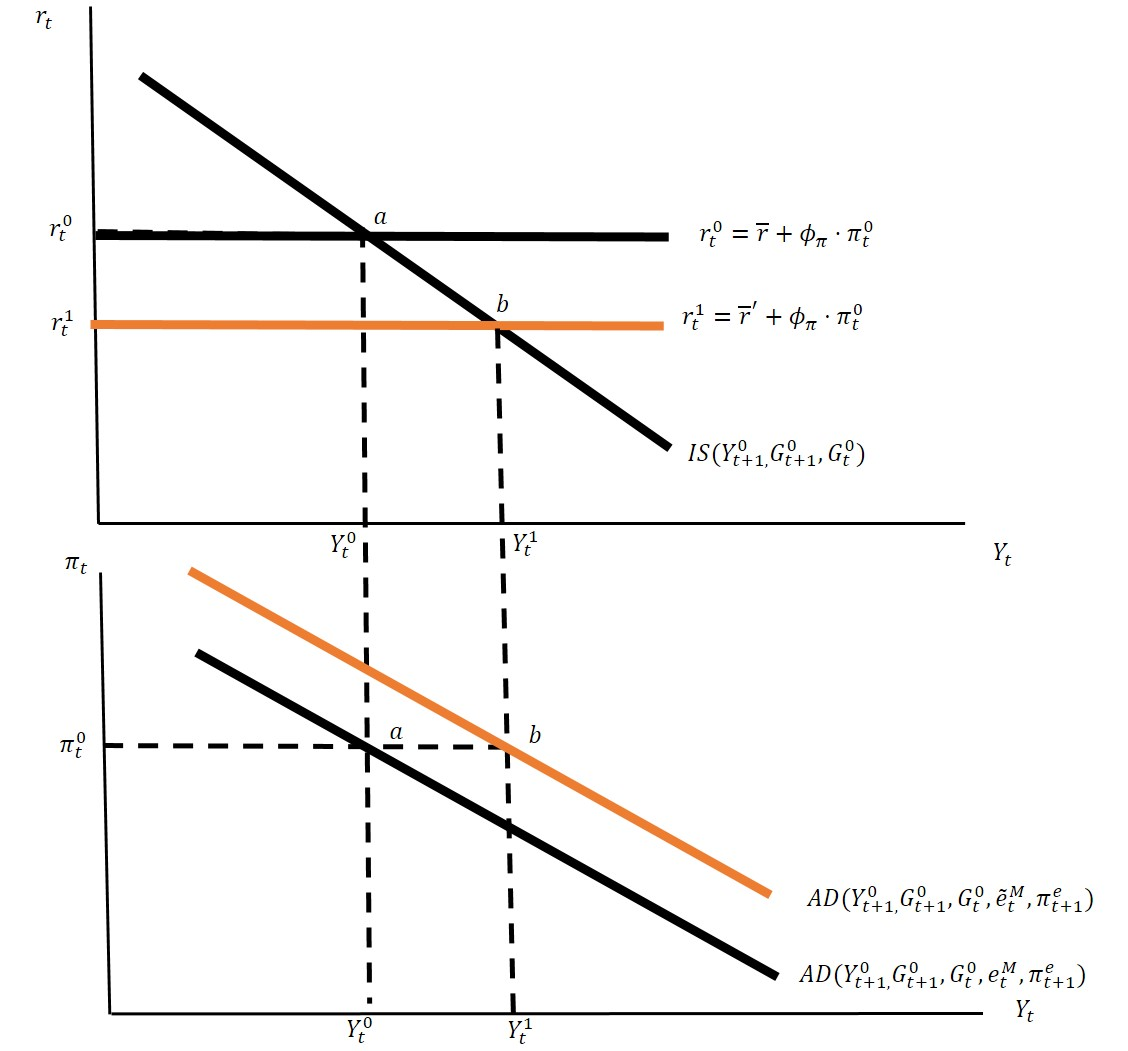
\includegraphics[width=\linewidth]{figAD2.jpg}
\end{column}
\begin{column}{0.5\textwidth}
\begin{itemize}
\item Think of a policy change that lowers the real rate for any given inflation:
\[
\bar r \downarrow \quad \text{(or a negative policy shock)}.
\]
\item \textbf{MP shifts down:} at any $\pi$, the policy rate is lower.
\item \textbf{AD implication:} lower $r$ boosts spending $\Rightarrow$ higher $Y$ at each $\pi$.
\end{itemize}

\vspace{0.3em}
\textbf{Key message:}\quad easier monetary policy shifts AD to the right.
\end{column}
\end{columns}
\end{frame}

%------------------------------------------------
\section[Supply]{Supply side: RBC $\Rightarrow$ AS}

%------------------------------------------------
\begin{frame}{Aggregate Supply: the FE benchmark}
\begin{columns}[onlytextwidth,T]
\begin{column}{0.55\textwidth}
\centering
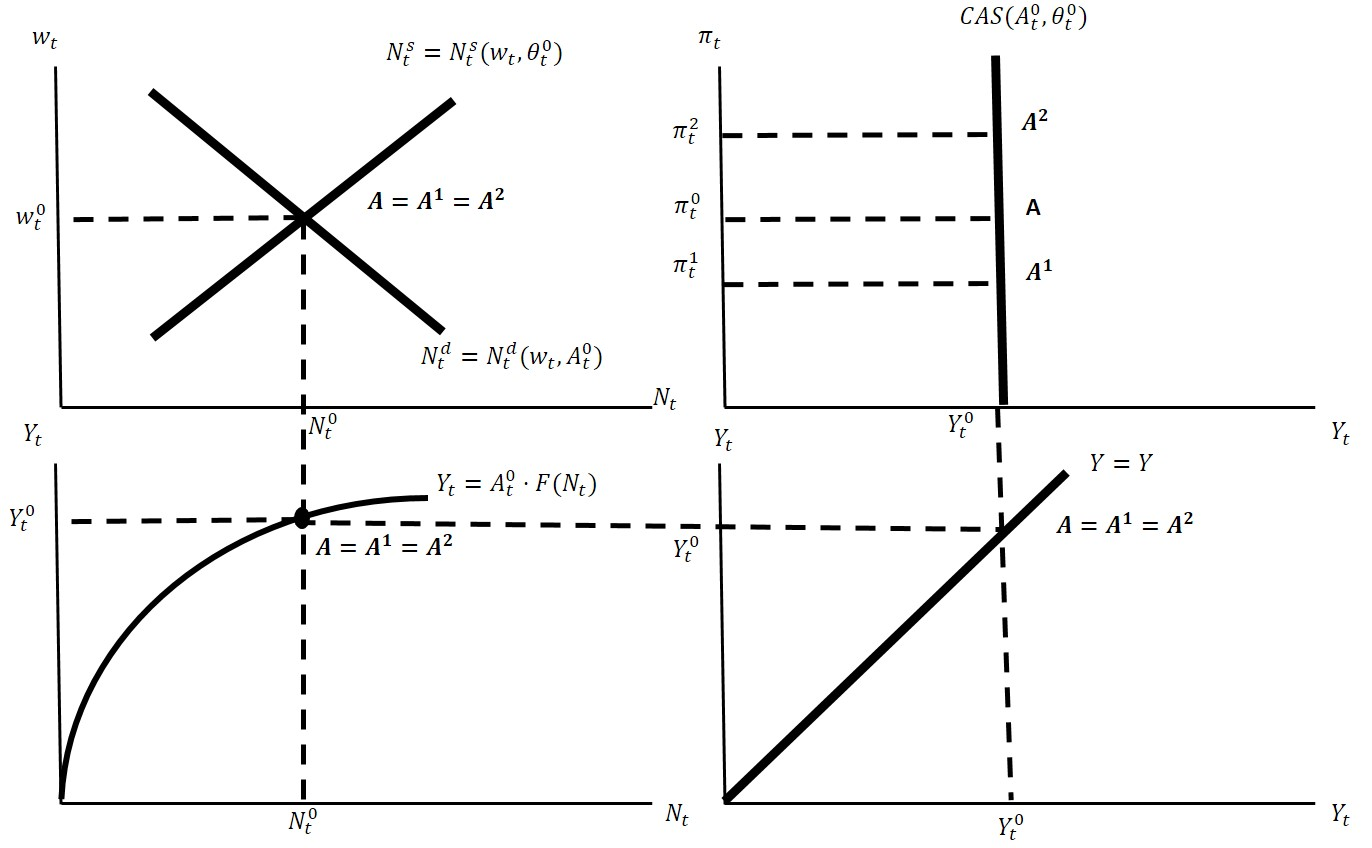
\includegraphics[width=\linewidth]{figAS.jpg}
\end{column}
\begin{column}{0.45\textwidth}
\begin{itemize}
\item \textbf{What this figure is doing:} re-plot the RBC supply block in $(\pi,Y)$ space.
\item In the classical/RBC model, output at a point in time is pinned down by
\begin{enumerate}
\item labor demand and labor supply,
\item the production function (productivity and capital).
\end{enumerate}
\item That level of output does not depend on inflation today.
\end{itemize}

\vspace{0.3em}
\textbf{Key message:}\quad Aggregate Supply (CAS) is vertical at the full-employment (potential) level of output.
\end{column}
\end{columns}
\end{frame}

%------------------------------------------------
\begin{frame}{CAS shifts left when productivity falls}
\begin{columns}[onlytextwidth,T]
\begin{column}{0.62\textwidth}
\centering
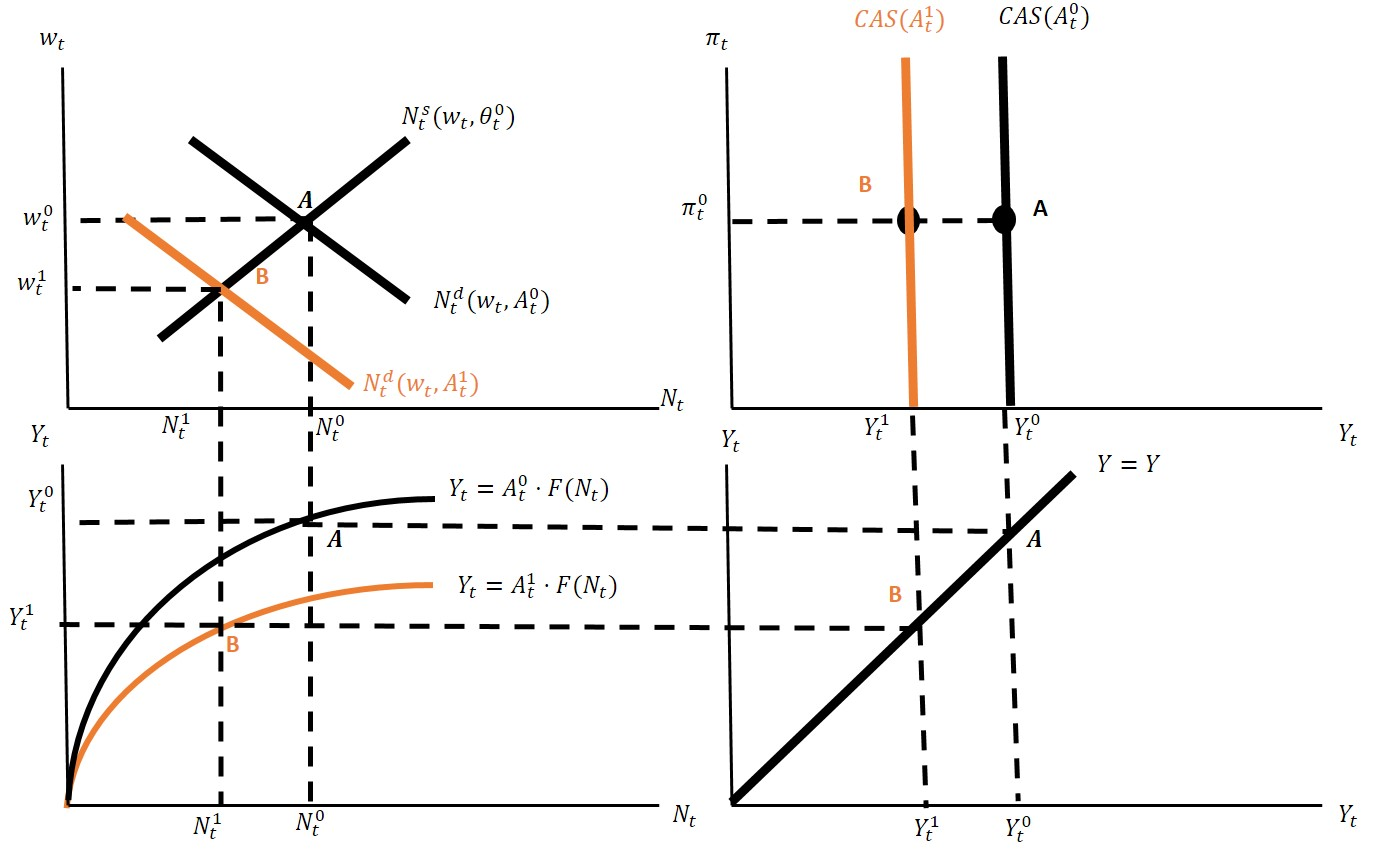
\includegraphics[width=\linewidth]{figAS1.jpg}
\end{column}
\begin{column}{0.38\textwidth}
\small
\begin{itemize}
\item \textbf{Shock:} $A\downarrow$ reduces the marginal product of labor.
\item Labor demand shifts left $\Rightarrow$ equilibrium employment falls.
\item With lower employment and productivity, full-employment output falls.
\end{itemize}

\vspace{0.3em}
\textbf{Key message:}\quad negative productivity shocks shift CAS left.
\end{column}
\end{columns}
\end{frame}

%------------------------------------------------
\begin{frame}{CAS shifts left when labor supply falls}
\begin{columns}[onlytextwidth,T]
\begin{column}{0.62\textwidth}
\centering
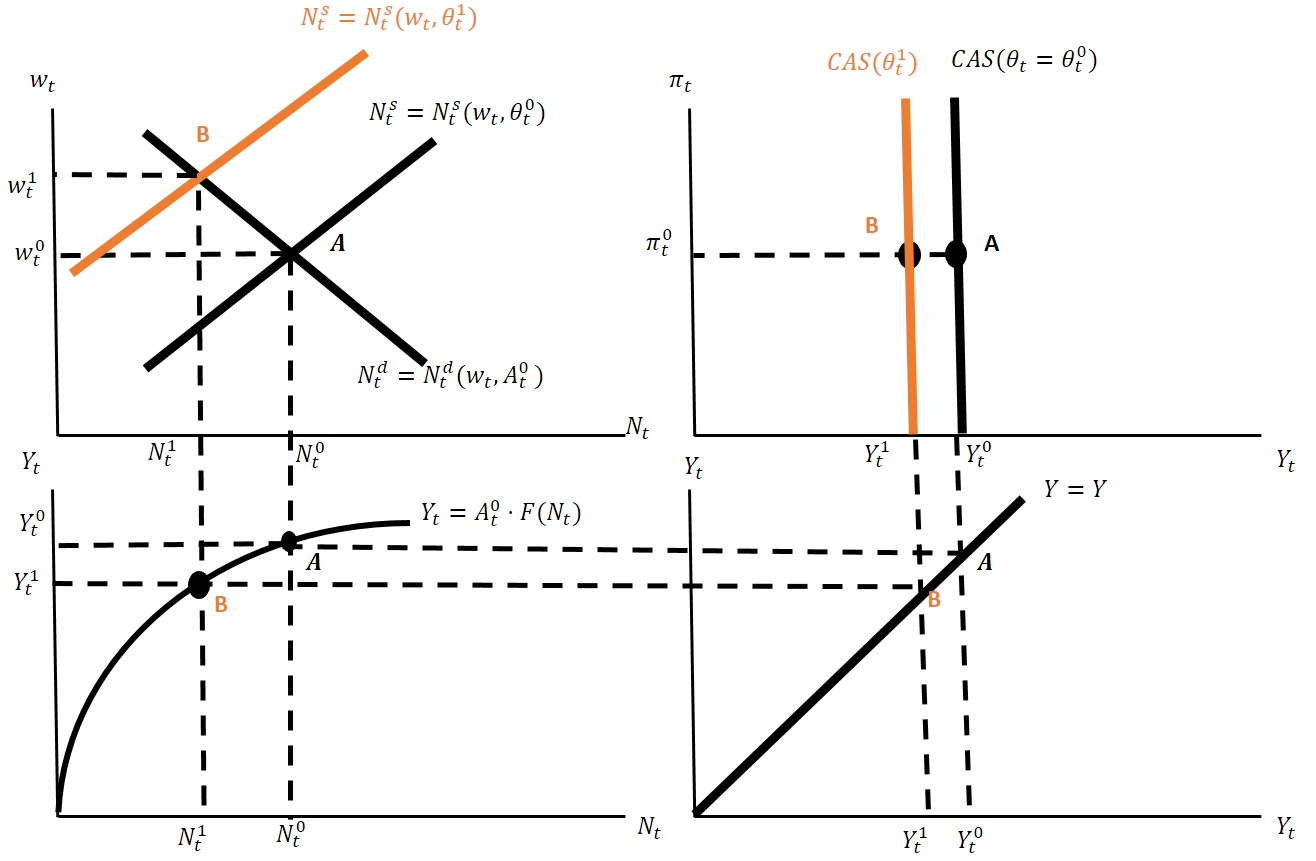
\includegraphics[width=\linewidth]{figAS2.jpg}
\end{column}
\begin{column}{0.38\textwidth}
\small
\begin{itemize}
\item \textbf{Shock:} $\theta\uparrow$ (a preference/distortion that reduces labor supply).
\item Labor supply shifts left $\Rightarrow$ equilibrium employment falls.
\item Lower employment reduces potential output.
\end{itemize}

\vspace{0.3em}
\textbf{Key message:}\quad labor supply disruptions also shift CAS left.
\end{column}
\end{columns}
\end{frame}

%------------------------------------------------
\begin{frame}{Demand vs supply shocks: the comovement test}
\begin{itemize}
\item \textbf{Demand shocks} (AD shifts) typically move output and inflation in the \textbf{same direction}.
\item \textbf{Supply shocks} (AS shifts) typically move output and inflation in \textbf{opposite directions}.
\end{itemize}

\vspace{0.4em}
\begin{enumerate}
\item AD $\uparrow$: $(Y\uparrow,\ \pi\uparrow)$
\item AS $\leftarrow$: $(Y\downarrow,\ \pi\uparrow)$ \quad (``stagflation'')
\end{enumerate}

\vspace{0.2em}
\textbf{Key message:}\quad this difference is the first diagnostic tool for inflation episodes.
\end{frame}

%------------------------------------------------
\section[Equilibrium]{AD--AS equilibrium and comparative statics}

%------------------------------------------------
\begin{frame}{AD--AS equilibrium (benchmark)}
\begin{columns}[onlytextwidth,T]
\begin{column}{0.62\textwidth}
\centering
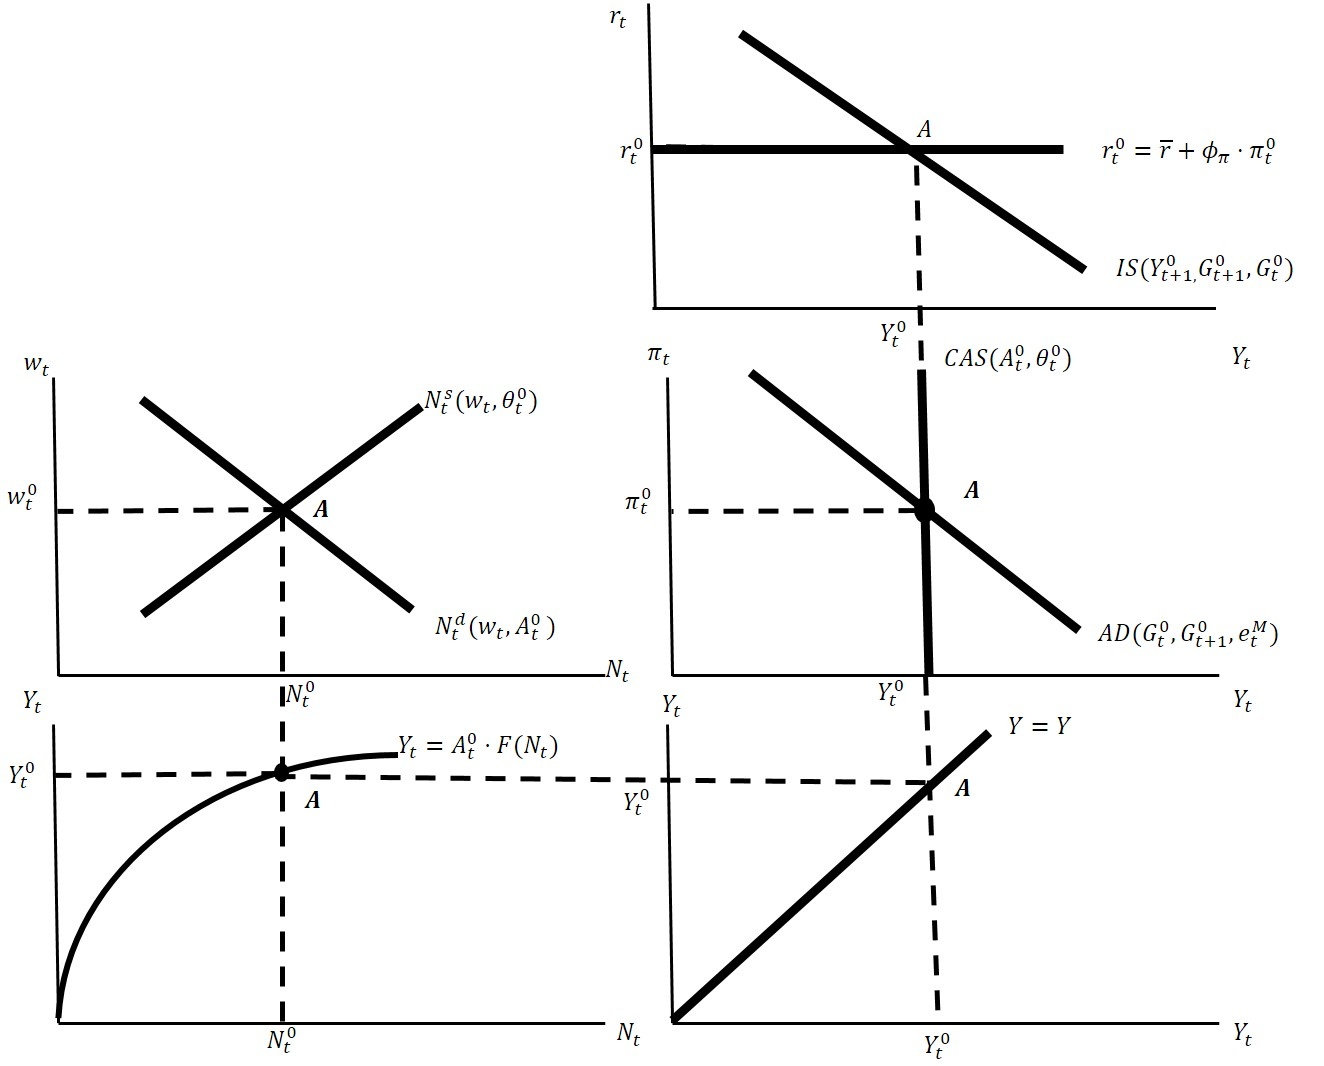
\includegraphics[width=\linewidth]{figADAS.jpg}
\end{column}
\begin{column}{0.38\textwidth}
\small
\begin{itemize}
\item \textbf{Equilibrium:} intersection of AD and CAS pins down $(\pi,Y)$.
\item \textbf{Interpretation:}
\begin{itemize}
\item AD tells you which $(\pi,Y)$ are consistent with IS + policy.
\item CAS tells you which $Y$ is feasible at full employment.
\end{itemize}
\item In this classical benchmark, $Y$ is pinned by CAS; AD determines $\pi$.
\end{itemize}

\vspace{0.3em}
\textbf{Key message:}\quad with flexible prices, output is supply-determined; inflation adjusts.
\end{column}
\end{columns}
\end{frame}

%------------------------------------------------
\begin{frame}{Demand shock: $G\uparrow$ (fiscal expansion)}
\begin{columns}[onlytextwidth,T]
\begin{column}{0.62\textwidth}
\centering
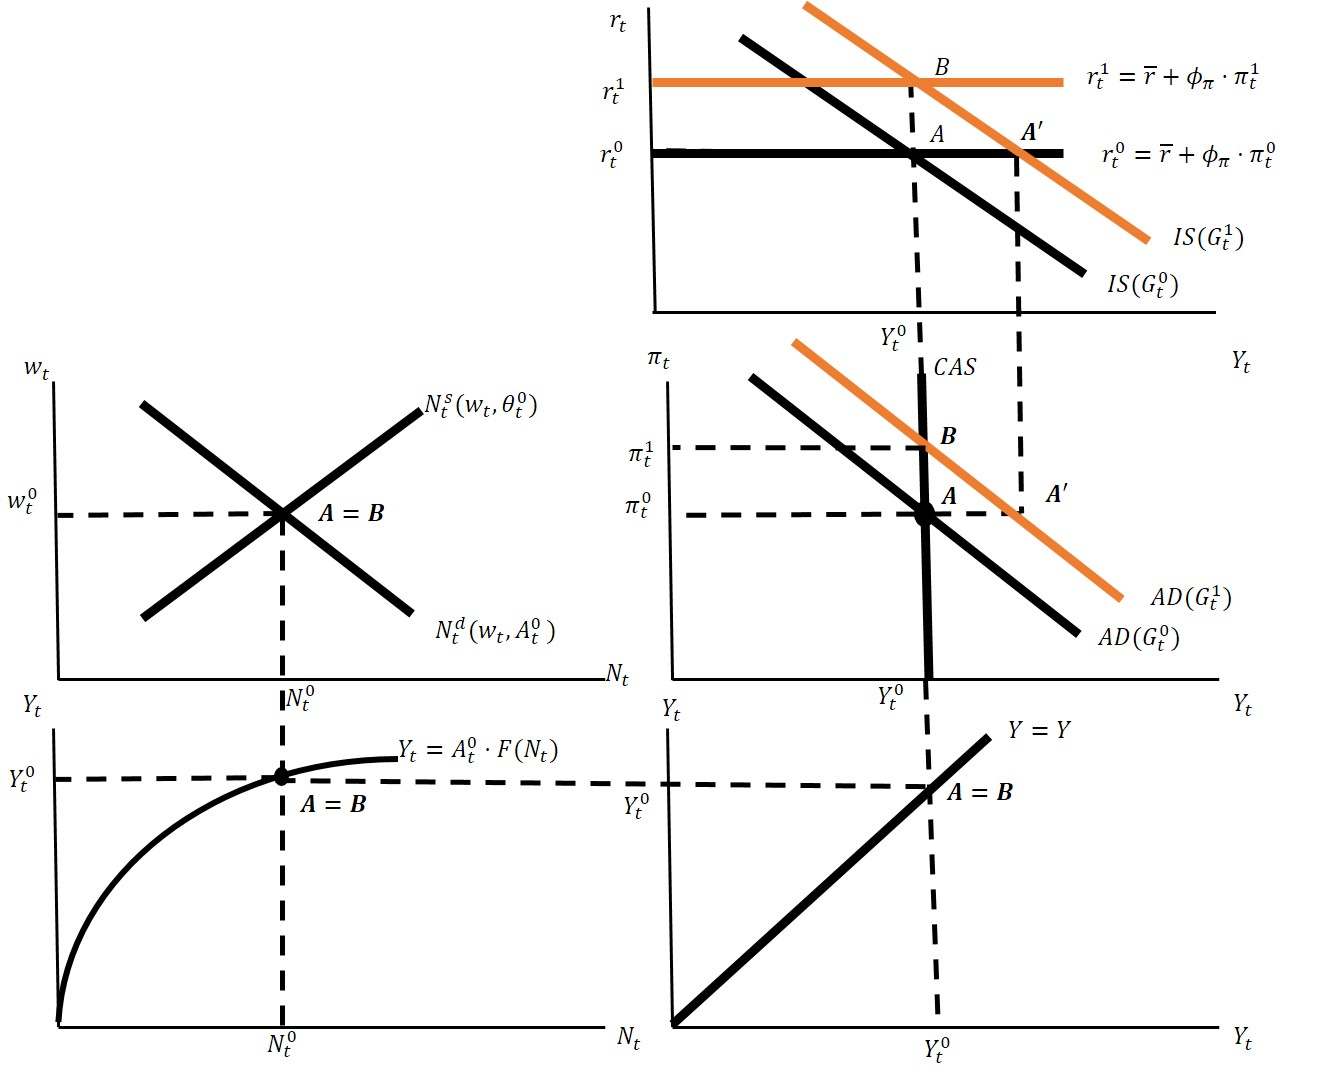
\includegraphics[width=\linewidth]{figADAS1.jpg}
\end{column}
\begin{column}{0.38\textwidth}
\small
\begin{itemize}
\item \textbf{Shift:} AD moves right.
\item \textbf{With vertical CAS:} output stays at potential $Y$.
\item \textbf{Adjustment:} inflation rises until MP raises $r$ enough to bring demand back to $Y$.
\end{itemize}

\vspace{0.3em}
\textbf{Key message:}\quad in the classical benchmark, fiscal expansion shows up as higher inflation, not higher output.
\end{column}
\end{columns}
\end{frame}

%------------------------------------------------
\begin{frame}{Demand shock: easier monetary policy}
\begin{columns}[onlytextwidth,T]
\begin{column}{0.62\textwidth}
\centering
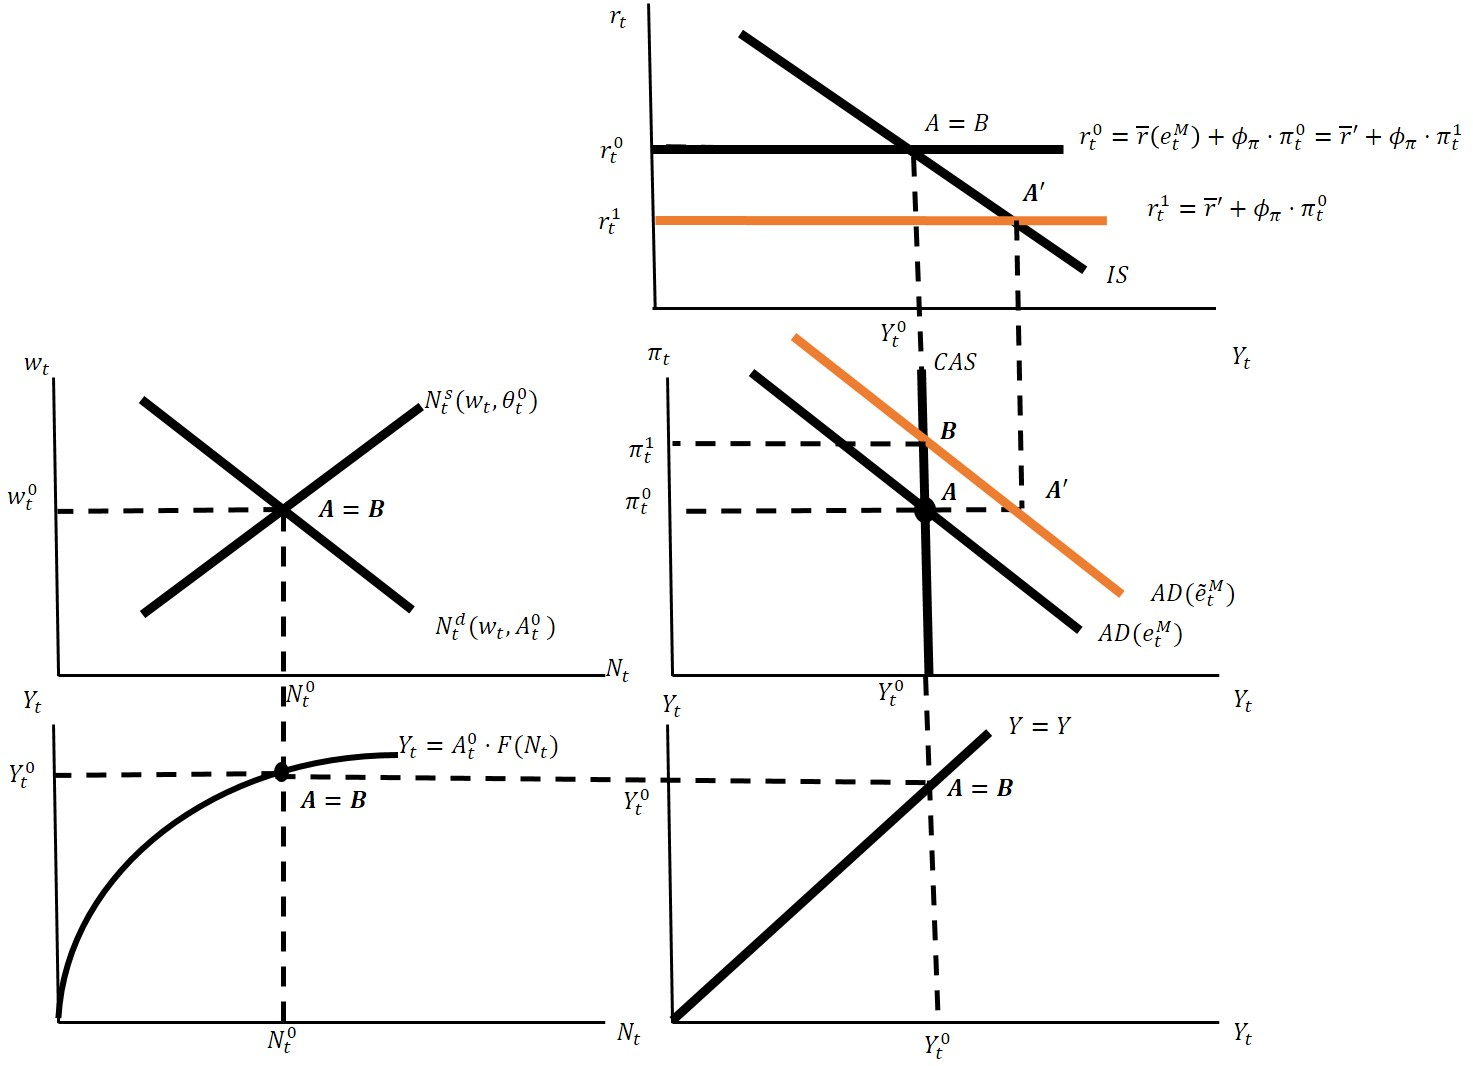
\includegraphics[width=\linewidth]{figADAS2.jpg}
\end{column}
\begin{column}{0.38\textwidth}
\small
\begin{itemize}
\item \textbf{Shift:} AD moves right (policy is easier for any given $\pi$).
\item \textbf{With vertical CAS:} output stays at potential $Y$.
\item \textbf{Adjustment:} inflation rises; MP then raises $r$ as $\pi$ rises.
\end{itemize}

\vspace{0.3em}
\textbf{Key message:}\quad money is neutral in the classical benchmark: policy changes mainly change inflation.
\end{column}
\end{columns}
\end{frame}

%------------------------------------------------
\begin{frame}{Supply shock: labor supply disruption ($\theta\uparrow$)}
\begin{columns}[onlytextwidth,T]
\begin{column}{0.62\textwidth}
\centering
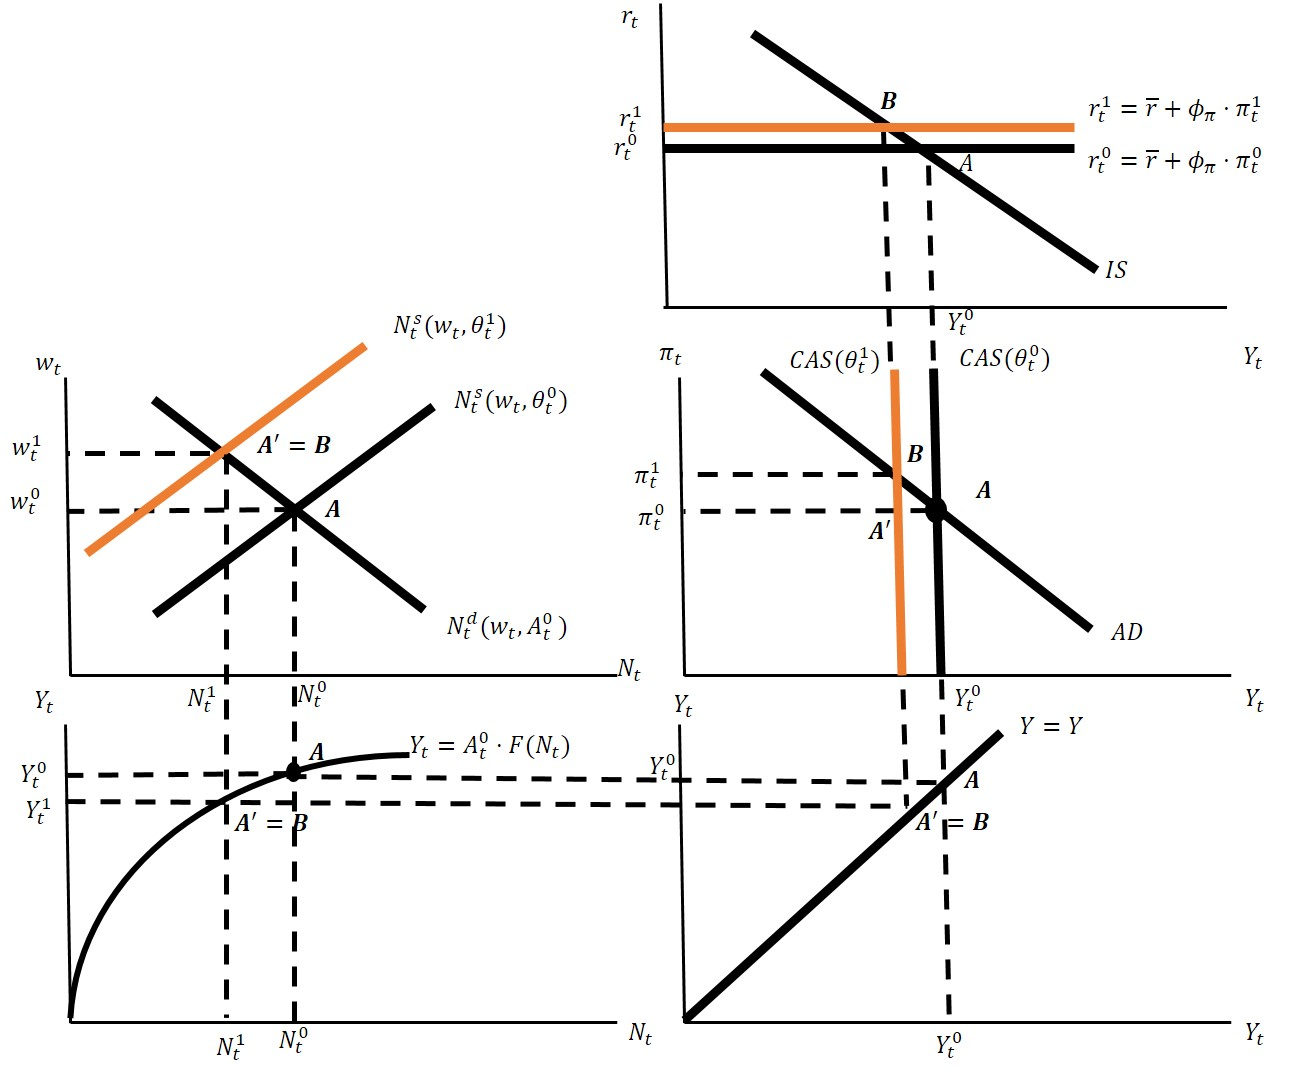
\includegraphics[width=\linewidth]{figADAS3.jpg}
\end{column}
\begin{column}{0.38\textwidth}
\small
\begin{itemize}
\item \textbf{Shift:} CAS moves left (potential output falls).
\item \textbf{Outcome:} output falls \emph{and} inflation rises.
\item \textbf{Policy response:} higher $\pi$ triggers a higher real rate via MP.
\end{itemize}

\vspace{0.3em}
\textbf{Key message:}\quad supply shocks generate stagflation: $(Y\downarrow,\ \pi\uparrow)$.
\end{column}
\end{columns}
\end{frame}

%------------------------------------------------
\begin{frame}{Supply shock: productivity declines ($A\downarrow$)}
\begin{columns}[onlytextwidth,T]
\begin{column}{0.62\textwidth}
\centering
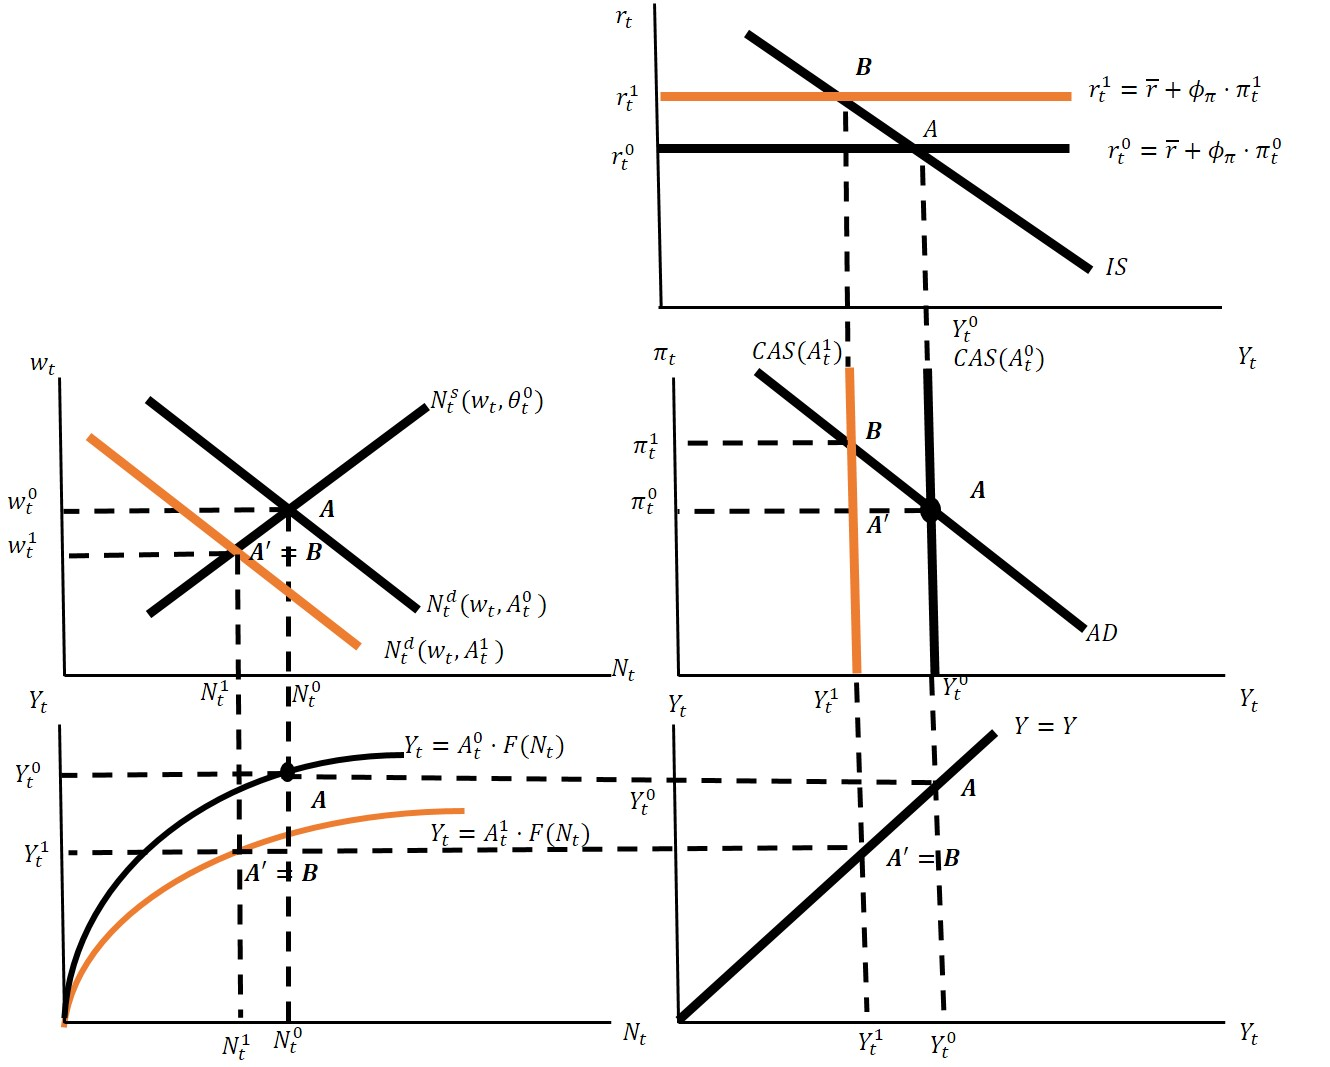
\includegraphics[width=\linewidth]{figADAS4.jpg}
\end{column}
\begin{column}{0.38\textwidth}
\small
\begin{itemize}
\item \textbf{Shift:} CAS moves left (potential output falls).
\item \textbf{Outcome:} lower output and higher inflation.
\item \textbf{Intuition:} less supply pushes up marginal costs / scarcity, raising inflation pressure.
\end{itemize}

\vspace{0.3em}
\textbf{Key message:}\quad negative productivity shocks also produce stagflation.
\end{column}
\end{columns}
\end{frame}

%------------------------------------------------
\begin{frame}{Summary table: shock $\Rightarrow$ shifts $\Rightarrow$ outcomes}
\small
\begin{center}
\begin{tabular}{lccc}
\toprule
\textbf{Shock} & \textbf{Curve shift} & \textbf{Output $Y$} & \textbf{Inflation $\pi$} \\
\midrule
$G\uparrow$ (fiscal)          & AD $\rightarrow$   & $\rightarrow$ & $\uparrow$ \\
Easier policy ($\bar r\downarrow$) & AD $\rightarrow$   & $\rightarrow$ & $\uparrow$ \\
$\theta\uparrow$ (labor supply down) & CAS $\leftarrow$ & $\downarrow$ & $\uparrow$ \\
$A\downarrow$ (productivity) & CAS $\leftarrow$     & $\downarrow$ & $\uparrow$ \\
\bottomrule
\end{tabular}
\end{center}

\vspace{0.2em}
\textbf{How to read this:}\quad demand shifts move $\pi$ with $Y$ fixed in the classical benchmark;\;
supply shifts move $Y$ and $\pi$ in opposite directions.
\end{frame}

%------------------------------------------------
\section{Wrap-up}

%------------------------------------------------
\begin{frame}{What this benchmark explains --- and what it cannot}
\begin{itemize}
\item \textbf{Explains well:}
\begin{itemize}
\item a clean diagnostic: demand vs supply shocks using $(Y,\pi)$ comovement,
\item why policy rules matter for demand (AD is policy-dependent),
\item why potential output shifts matter for inflation.
\end{itemize}
\item \textbf{Cannot explain (yet):}
\begin{itemize}
\item persistent output gaps (because CAS is vertical),
\item gradual disinflation without large output losses,
\item the central role of expectations in inflation dynamics.
\end{itemize}
\end{itemize}

\vspace{0.3em}
\textbf{Key message:}\quad this classical AD--AS is a benchmark; next we add nominal rigidities (New Keynesian model).
\end{frame}

%------------------------------------------------
\begin{frame}{Preview: what changes with sticky prices (next lecture)}
\begin{itemize}
\item With price/wage rigidity, the supply side is no longer vertical in the short run.
\item Then AD shifts can raise output \emph{and} inflation in the short run.
\item We will replace ``CAS'' with a \textbf{Phillips curve}:
\[
\pi_t = \beta \mathbb{E}_t[\pi_{t+1}] + \kappa (Y_t - Y_t^{*}) + u_t.
\]
\item That introduces expectations and persistence --- the core of modern inflation analysis.
\end{itemize}

\vspace{0.3em}
\textbf{Key message:}\quad NK = AD (IS + policy rule) + AS (Phillips curve) + expectations.
\end{frame}

%------------------------------------------------
\begin{frame}{Next time}
\Large
\begin{itemize}
\item Short-run aggregate supply with sticky prices
\item Phillips curve logic and inflation persistence
\item Monetary policy rules and the ``Taylor principle'' (why the anchor matters)
\end{itemize}
\end{frame}

\end{document}
